\newpage

\chapter{Měření charakteristik zdroje}

Tato kapitola se zaměřuje na experimentální ověření klíčových charakteristik navrženého proudového zdroje.
Podrobně popisuje provedená měření stejnosměrného i střídavého proudového výstupu, dynamické odezvy na změny zátěže, účinnosti a ztrát,
teplotního zatížení a úrovně generovaného šumu a rušení. Cílem těchto měření bylo kvantifikovat výkonové parametry zdroje,
posoudit jeho stabilitu a kvalitu výstupního signálu v různých provozních podmínkách.
Výsledky těchto analýz poskytují komplexní pohled na funkční vlastnosti a limity navrženého zařízení.

\section{Stejnosměrný proudový výstup}


Ve stejnosměrném režimu byly provedeny měření výstupního proudu, jeho efektivní hodnoty a zvlnění.
Cílem bylo zhodnotit stabilitu výstupu při různých vstupních napětích a zátěžových podmínkách
a jeho výsledky jsou uvedeny v tabulce \ref{tab:dc_measurements}.

\begin{table}[htbp]
	\centering
	\caption{Výsledky měření výstupního proudu, zvlnění a efektivní hodnoty}
	\setlength{\tabcolsep}{4pt}
	\renewcommand{\arraystretch}{1.2}

	\begin{tabular}{|c|*{8}{c|}}
		\hline
		\multicolumn{9}{|c|}{$U_{\text{vstupní}} = \SI{12}{\volt}$ pro \SI{1}{\ohm} \text{zátěž s indukčností }\SI{720}{\micro\henry}} \\
		\hline
		$I_{\text{nastavený}}$ (\si{\ampere}) & -8,00 & -4,00 & -1,00 & -0,10 & 0,10  & 1,00 & 4,00  & 8,00                            \\
		\hline
		$I_{\text{výstup}}$ (\si{\ampere})    & -8,32 & -4,16 & -1,02 & -0,10 & 0,15  & 0,99 & 4,07  & 8,21                            \\
		\hline
		$I_{\text{zvlnění}}$ (\si{\ampere})   & 0,03  & 0,02  & 0,01  & 0,01  & 0,02  & 0,01 & 0,02  & 0,03                            \\
		\hline
		Zvlnění (\%)                          & 0,35  & 0,55  & 1,38  & 10,58 & 11,69 & 1,42 & 0,54  & 0,32                            \\
		\hline
		$I_{\text{RMS}}$ (\si{\ampere})       & 8,32  & 4,16  & 1,02  & 0,10  & 0,16  & 0,99 & 4,07  & 8,21                            \\
		\hline

		\multicolumn{9}{|c|}{$U_{\text{vstupní}} = \SI{48}{\volt}$ pro \SI{1}{\ohm} \text{zátěž s indukčností }\SI{720}{\micro\henry}} \\
		\hline
		$I_{\text{nastavený}}$ (\si{\ampere}) & -8,00 & -4,00 & -1,00 & -0,10 & 0,10  & 1,00 & 4,00  & 8,00                            \\
		\hline
		$I_{\text{výstup}}$ (\si{\ampere})    & -8,36 & -4,36 & -1,06 & -0,24 & 0,14  & 1,04 & 4,35  & 8,42                            \\
		\hline
		$I_{\text{zvlnění}}$ (\si{\ampere})   & 1,29  & 0,47  & 0,10  & 0,05  & 0,02  & 0,08 & 0,44  & 1,35                            \\
		\hline
		Zvlnění (\%)                          & 15,42 & 10,77 & 9,26  & 18,44 & 17,14 & 7,98 & 10,18 & 16,03                           \\
		\hline
		$I_{\text{RMS}}$ (\si{\ampere})       & 8,46  & 4,39  & 1,06  & 0,25  & 0,14  & 1,04 & 4,38  & 8,53                            \\
		\hline

		\multicolumn{9}{|c|}{$U_{\text{vstupní}} = \SI{48}{\volt}$ pro \SI{3}{\ohm} \text{zátěž s indukčností }\SI{720}{\micro\henry}} \\
		\hline
		$I_{\text{nastavený}}$ (\si{\ampere}) & -8,00 & -4,00 & -1,00 & -0,10 & 0,10  & 1,00 & 4,00  & 8,00                            \\
		\hline
		$I_{\text{výstup}}$ (\si{\ampere})    & -8,20 & -4,16 & -1,08 & -0,24 & 0,11  & 0,91 & 4,00  & 7,90                            \\
		\hline
		$I_{\text{zvlnění}}$ (\si{\ampere})   & 0,68  & 0,24  & 0,04  & 0,04  & 0,03  & 0,05 & 0,29  & 0,62                            \\
		\hline
		Zvlnění (\%)                          & 8,27  & 5,66  & 3,87  & 15,68 & 23,42 & 5,71 & 7,17  & 7,85                            \\
		\hline
		$I_{\text{RMS}}$ (\si{\ampere})       & 8,23  & 4,16  & 1,08  & 0,24  & 0,11  & 0,91 & 4,01  & 7,92                            \\
		\hline
	\end{tabular}
	\label{tab:dc_measurements}
\end{table}

Graf \ref{fig::zavislost_proudu} ukazuje závislost výstupního proudu na nastaveném proudu pro různá vstupní napětí.
Zatěžovací charakteristika zdroje je znázorněna v grafu \ref{fig::zatezovaci_char}
a relativní zvlnění výstupního proudu je zobrazeno v grafu \ref{fig::dc_zvlneni}.
Měření ukazují, že výstupní proud dobře kopíruje nastavenou hodnotu s minimální odchylkou.
Největší relativní zvlnění se projevilo při malých proudech, což je běžné u spínaných napájecích zdrojů,
kde je dominantní šum a nelinearity regulace.



\begin{figure}[htpb]
	\centering
	\includegraphics[width=0.95\textwidth]{kapitola5/Figures/Graf1_Vystupni_charakteristika.png} % Cesta k souboru s diagramem
	\caption{Velikost výstupního proudu v závislosti na nastaveném proudu}
	\label{fig::zavislost_proudu}
\end{figure}


\begin{figure}[htpb]
	\centering
	\includegraphics[width=0.95\textwidth]{kapitola5/Figures/Graf2_Zatezova_char_proud.png} % Cesta k souboru s diagramem
	\caption{Zatěžovací charakteristika zdroje}
	\label{fig::zatezovaci_char}
\end{figure}


\begin{figure}[htpb]
	\centering
	\includegraphics[width=0.95\textwidth]{kapitola5/Figures/Graf3_Zvlneni_proudu.png} % Cesta k souboru s diagramem
	\caption{Relativní zvlnění výstupního proudu v závislosti na nastaveném proudu a vstupním napětí}
	\label{fig::dc_zvlneni}
\end{figure}

\section{Střídavý proud}


Pro určení kvalitativních vlastností výstupního střídavého proudu byla změřena efektivní hodnota výstupního proudu
a spektrum výstupního signálu pro různé tvary signálu, nastavené proudy a vstupní napětí.
Na základě těchto měření bylo určeno celkové harmonické zkreslení (THD) výstupního proudu,
které je znázorněno v grafu \ref{fig::ac_THD}.

Celkové harmonické zkreslení (THD) slouží jako ukazatel kvality výstupního střídavého proudu.
Pro ideální sinusový signál by THD mělo být co nejnižší (blízko \SI{0}{\percent}).
Naproti tomu ideální obdélníkový a trojúhelníkový průběh vykazují přirozeně vyšší THD hodnoty,
asice \SI{48.3}{\percent} a \SI{12,1}{\percent}.

\begin{table}[htbp]
	\centering
	\caption{Výsledky měření výstupního střídavého proudu, základní harmonické a harmonického zkreslení pro různé tvary signálu}
	\setlength{\tabcolsep}{4pt}
	\renewcommand{\arraystretch}{1.2}
	\begin{tabular}{|c|*{9}{c|}}
		\hline
		                                  & \multicolumn{3}{c|}{\textbf{Harmonický 10 Hz}} & \multicolumn{3}{c|}{\textbf{Obdélníkový 10 Hz}} & \multicolumn{3}{c|}{\textbf{Trojúhelníkový 10 Hz}}                                                 \\
		\hline
		$I_{\text{nast.}}$ (\si{\ampere}) & 1,00                                           & 4,00                                            & 8,00                                               & 1,00  & 4,00  & 8,00  & 1,00  & 4,00  & 8,00  \\
		\hline

		\multicolumn{10}{|c|}{$U_{\text{vstupní}} = \SI{12}{\volt}$}                                                                                                                                                                              \\
		\hline
		$I_{\text{ef}}$ (\si{\ampere})    & 0,75                                           & 2,94                                            & 5,80                                               & 1,03  & 4,06  & 8,11  & 0,60  & 2,37  & 4,72  \\
		\hline
		$I_1$ (\si{\deci\bel})            & -2,52                                          & 9,26                                            & 15,08                                              & -0,61 & 11,29 & 17,29 & -4,63 & 7,43  & 13,41 \\
		\hline
		$I_1$ (\si{\ampere})              & 0,75                                           & 2,90                                            & 5,67                                               & 0,93  & 3,67  & 7,32  & 0,59  & 2,35  & 4,68  \\
		\hline
		THD (\%)                          & 10,28                                          & 15,67                                           & 21,14                                              & 47,49 & 47,65 & 47,69 & 18,68 & 11,51 & 12,64 \\
		\hline

		\multicolumn{10}{|c|}{$U_{\text{vstupní}} = \SI{48}{\volt}$}                                                                                                                                                                              \\
		\hline
		$I_{\text{ef}}$ (\si{\ampere})    & 0,77                                           & 3,04                                            & 5,78                                               & 1,07  & 4,16  & 8,07  & 0,63  & 2,47  & 4,80  \\
		\hline
		$I_1$ (\si{\deci\bel})            & -2,53                                          & 9,31                                            & 14,78                                              & -0,52 & 11,26 & 17,01 & -4,13 & 7,75  & 13,51 \\
		\hline
		$I_1$ (\si{\ampere})              & 0,75                                           & 2,92                                            & 5,48                                               & 0,94  & 3,65  & 7,09  & 0,62  & 2,44  & 4,74  \\
		\hline
		THD (\%)                          & 21,86                                          & 28,95                                           & 33,37                                              & 54,33 & 54,43 & 54,44 & 20,06 & 15,56 & 16,37 \\
		\hline
	\end{tabular}
	\label{tab:ac_measurements}
\end{table}


\begin{figure}[htpb]
	\centering
	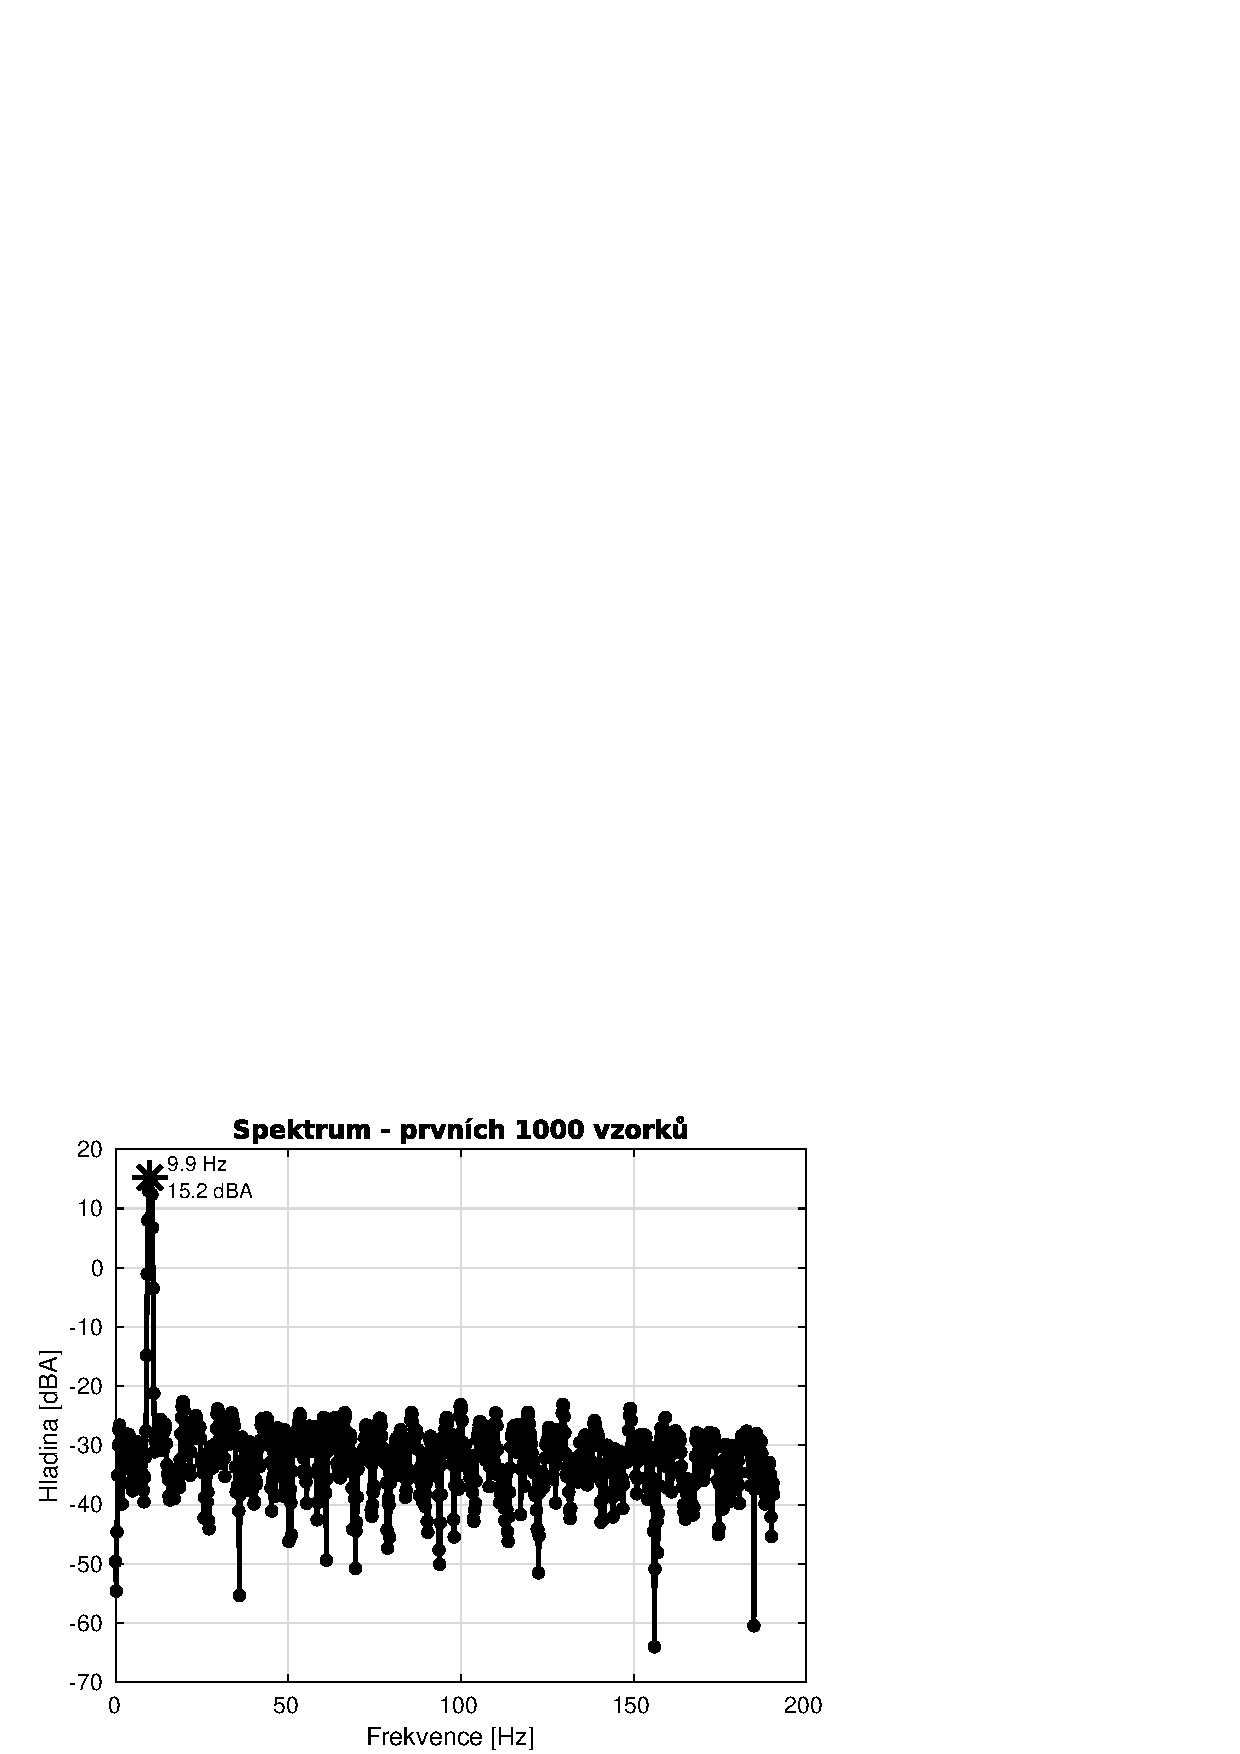
\includegraphics[width=0.95\textwidth]{kapitola5/Figures/sin10hz_8amp_12V.png}
	\caption{Část spektra výstupního proudu do \SI{200}{Hz} pro sinusový průběh \SI{10}{Hz} při \SI{8}{A} a \SI{12}{V}}
	\label{fig::spectrum_sin10hz}
\end{figure}

\begin{figure}[htpb]
	\centering
	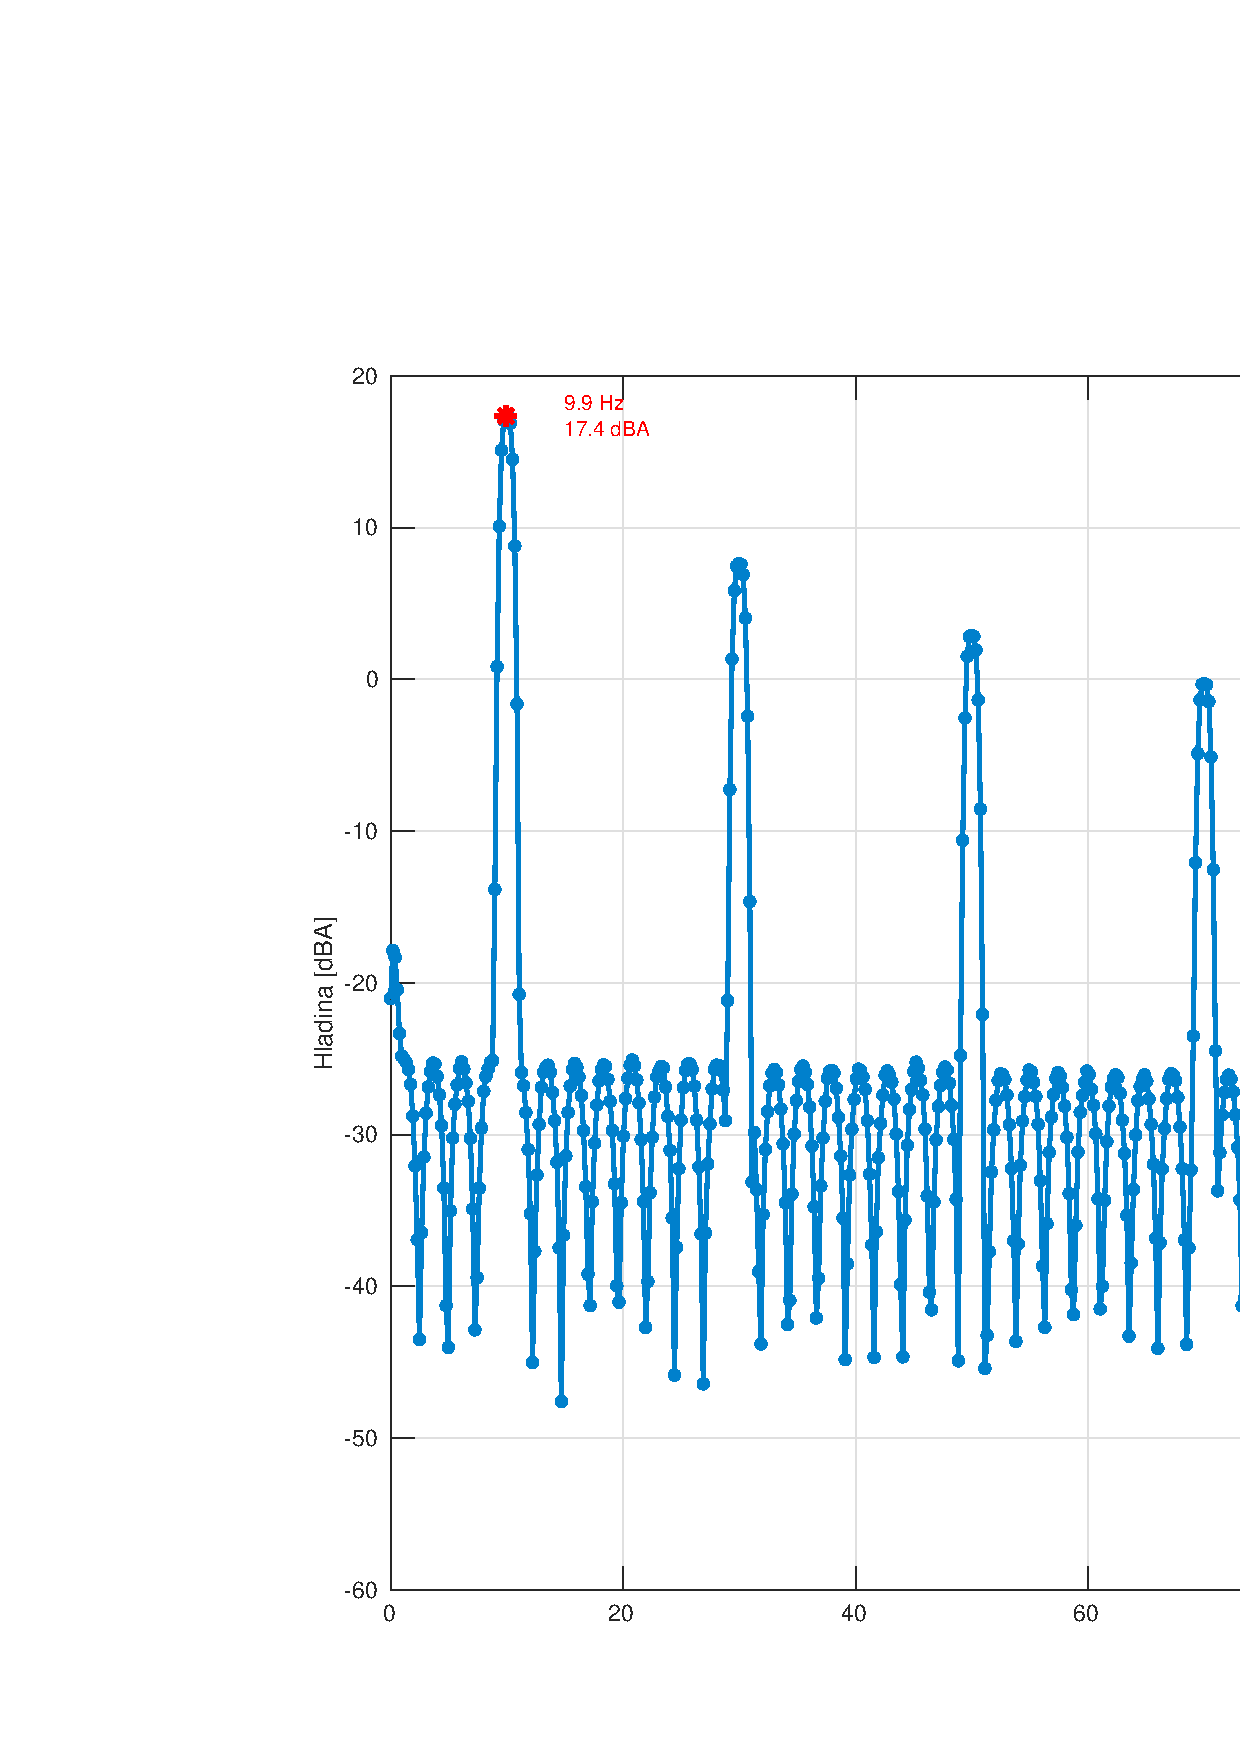
\includegraphics[width=0.95\textwidth]{kapitola5/Figures/SQ10HZ_8A_12V.png}
	\caption{Část spektra výstupního proudu do \SI{200}{Hz} pro obdélníkový průběh \SI{10}{Hz} při \SI{8}{A} a \SI{12}{V}}
	\label{fig::spectrum_SQ10HZ}
\end{figure}

\begin{figure}[htpb]
	\centering
	\includegraphics[width=0.95\textwidth]{kapitola5/Figures/nastavena_realna_amplituda.png} % Cesta k souboru s diagramem
	\caption{Změřená závislost nastaveného a reálné amplitudy}
	\label{fig::ac_first_harmonic}
\end{figure}

\begin{figure}[htpb]
	\centering
	\includegraphics[width=0.95\textwidth]{kapitola5/Figures/THD_AC.png} % Cesta k souboru s diagramem
	\caption{Vypočítané celkové harmonické zkreslení (THD) pro různé tvary signálu}
	\label{fig::ac_THD}
\end{figure}

Výsledky potvrzují očekávaný trend – sinusový průběh má nejnižší zkreslení,
zatímco obdélníkový vykazuje nejvyšší hodnoty THD.
Zjištěné hodnoty THD jsou dostačujicí pro potřeby napájení elektromagnetických aktuátorů.

\section{Dynamická odezva}

Pro posouzení dynamické odezvy zdroje na rychlé změny zátěže byly provedeny skokové změny odporu,
viz \oref{fig::dynamic_load_hlower} a \oref{fig::dynamic_load_higher}.
Reakce byla snímána pomocí osciloskopu při konstantním nastavení proudu \SI{3}{\ampere}.
Výsledky demonstrují schopnost regulátoru rychle stabilizovat výstup.
Tato zátěž (resp. proud) byla zvolena, protože představuje maximální proud,
který je zdroj schopen dodat při vstupním napětí \SI{12}{\volt}, aniž by byl výstupní proud omezen pouze odporem zátěže.
Vstupní napětí \SI{12}{\volt} bylo zvoleno proto,
že při tomto napětí je výstupní proud nejméně ovlivněn rušením a skoková změna zátěže je na osciloskopu nejlépe pozorovatelná.
Zdroj vykazuje rychlou a stabilní reakci s minimálním přechodovým zvlněním.

\begin{figure}[htpb]
	\centering
	\includegraphics[width=0.95\textwidth]{kapitola5/Figures/DUPRR_12V_3A.png} % Cesta k souboru s diagramem
	\caption{Reakce na skokové zvýšení odporu zátěže z $\SI{0.4}{\ohm}$ na $\SI{3.4}{\ohm}$ při konstantním nastaveném proudu $\SI{3}{\ampere}$}
	\label{fig::dynamic_load_higher}
\end{figure}

\begin{figure}[htpb]
	\centering
	\includegraphics[width=0.95\textwidth]{kapitola5/Figures/DYNLOWER_12V.png} % Cesta k souboru s diagramem
	\caption{Reakce na skokové snížení odporu zátěže z $\SI{3.4}{\ohm}$ na $\SI{0.4}{\ohm}$ při konstantním nastaveném proudu $\SI{3}{\ampere}$}
	\label{fig::dynamic_load_hlower}
\end{figure}


\section{Účinnost a ztráty}

Účinnost byla určena jako poměr výstupního a vstupního výkonu.
Při zatížení \SI{8}{\ampere} a napětí \SI{31}{\volt} dosahuje zdroj maximální účinnosti \SI{91.66}{\percent}.
Nižší účinnost při malých výkonech je způsobena relativně vyššími ztrátami v řídicích a spínacích obvodech,
které se v tomto režimu stávají dominantními.
Vstupní výkon byl měřen pomocí laboratorního zdroje s integrovaným měřením dodávaného výkonu.
Výstupní zdánlivý výkon byl odvozen z efektivní hodnoty napětí a proudu pomocí dvou multimetrů.
Zátěž se známou indukčností a odporem umožnila výpočet činného výkonu dodávaného do zátěže (tabulka \ref{tab:efficiency_dc}).

\begin{table}[htbp]
    \centering
    \caption{Výsledky měření účinnosti ve stejnosměrném režimu}
    \setlength{\tabcolsep}{10pt}
    \renewcommand{\arraystretch}{1.2}
    
    \begin{tabular}{|c|*{3}{c|}}
        \hline
        \multicolumn{4}{|c|}{\textbf{Stejnosměrný režim (DC)}} \\
        \hline
        \multicolumn{4}{|c|}{$U_{\text{vstupní}} = \SI{12}{\volt}$ pro zátěž $R = \SI{1,2}{\ohm}$ o indukčnosti $\SI{720}{\micro\henry}$} \\
        \hline
        Nastavený proud $I_{\text{nast.}}$ (\si{\ampere}) & 1,00 & 4,00 & 8,00 \\
        \hline
        Výstupní proud $I_{\text{výst.}}$ (\si{\ampere}) & 0,90 & 3,93 & 8,06 \\
        \hline
        Výstupní výkon $P_{\text{výst.}}$ (\si{\watt}) & 0,97 & 18,49 & 77,96 \\
        \hline
        Vstupní výkon $P_{\text{vst.}}$ (\si{\watt}) & 1,99 & 22,28 & 88,80 \\
        \hline
        Účinnost $\eta$ (\%) & 48,57 & 82,97 & 87,79 \\
        \hline
        
        \multicolumn{4}{|c|}{$U_{\text{vstupní}} = \SI{31}{\volt}$ pro zátěž $R = \SI{1,2}{\ohm}$ o indukčnosti $\SI{720}{\micro\henry}$} \\
        \hline
        Nastavený proud $I_{\text{nast.}}$ (\si{\ampere}) & 1,00 & 4,00 & 8,00 \\
        \hline
        Výstupní proud $I_{\text{výst.}}$ (\si{\ampere}) & 0,90 & 4,30 & 8,36 \\
        \hline
        Výstupní výkon $P_{\text{výst.}}$ (\si{\watt}) & 0,96 & 22,19 & 83,87 \\
        \hline
        Vstupní výkon $P_{\text{vst.}}$ (\si{\watt}) & 2,33 & 27,00 & 91,50 \\
        \hline
        Účinnost $\eta$ (\%) & 41,29 & 82,18 & 91,66 \\
        \hline
    \end{tabular}
    \label{tab:efficiency_dc}
\end{table}

\begin{figure}[htpb]
	\centering
	\includegraphics[width=0.95\textwidth]{kapitola5/Figures/Analyza_ucinnosti_DC.png} % Cesta k souboru s diagramem
	\caption{Změřená účinnost zdroje ve stejnosměrném režimu}
	\label{fig::ac_efficiency}
\end{figure}


\section{Teplotní zatížení}

Po hodině provozu při výstupním proudu \SI{8}{\ampere} a
napájecím napětí \SI{48}{\volt} dosáhla teplota na povrchu výkonových tranzistorů hodnoty \SI{92,4}{\degreeCelsius},
což je s rezervou v mezích doporučených výrobcem, viz \cite{ISC080N10NM6_ds}.

\section{Šum a rušení}

Měření v EMC komoře ukázala,
že bez dodatečných filtračních obvodů zdroj nesplňuje požadavky norem na elektromagnetickou kompatibilitu,
viz (viz přílohy \ref{priloha:mereni_emc_standby} a \ref{priloha:mereni_emc_on}).
Nejproblematičtější jsou přechodové jevy při spínání výkonových tranzistorů,
které generují výrazné vysokofrekvenční složky.
Návrh vhodného LC filtru na vstupu a výstupu spolu s použitím snubberů může tyto projevy významně omezit.
Na základě měření v EMC komoře je však možné určit vhodné parametry pro návrh filtru.
